\section{Load Case}
\label{sec:loading}

\textit{The first step of every structural analysis problem is defining the exact problem. To do that free body diagrams are constructed to show geometry, dimensions and acting forces and moments. Then, an accurate and detailed description of the load case is required to ensure realistic results.}

\subsection{Loading scenario}
The concerned loading case of the aileron is caused by the critical loading scenario of the Fokker 100. This scenario is a combination of a couple elements: The aileron is deflected to it's maximum potential upward deflection which is 30 degrees. Also, the aerodynamic loading of the wing is at the limit load. Lastly, one of the actuators used to control the aileron is jammed while the second actuator is giving a discrete load in the negative z-direction.

\subsection{Reference frame}
The reference frame used for the model has its x-axis in span wise direction, pointing towards the tip of the undeformed main wing. The z-axis is in chord wise direction, pointing towards the leading edge. Finally, the y-axis is directed upwards, orthogonal to the aileron surface. This reference frame is visualised in \figautoref{reference_frame}.

\begin{figure}[H]
    \centering
    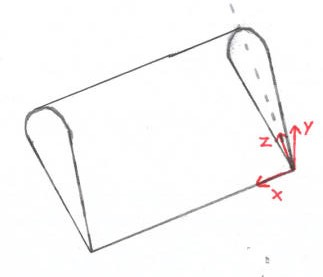
\includegraphics[width=4.5cm]{Images/reference_frame.jpg}
    \caption{Reference frame}
    \label{reference_frame}
\end{figure}


\subsection{Geometry and specifications}
The geometry of the aileron is visualised in \figautoref{fig:Dimensions_top_view}, \figautoref{fig:Dimensions_side_view} and \figautoref{fig:Dimensions_back_view}. The important dimensions are labeled with parameters. These parameters are further defined for our Fokker 100 airplane in \figautoref{ParametersaileronF100}.



\begin{figure}[H]
\begin{minipage}[b]{0.45\linewidth}
\centering
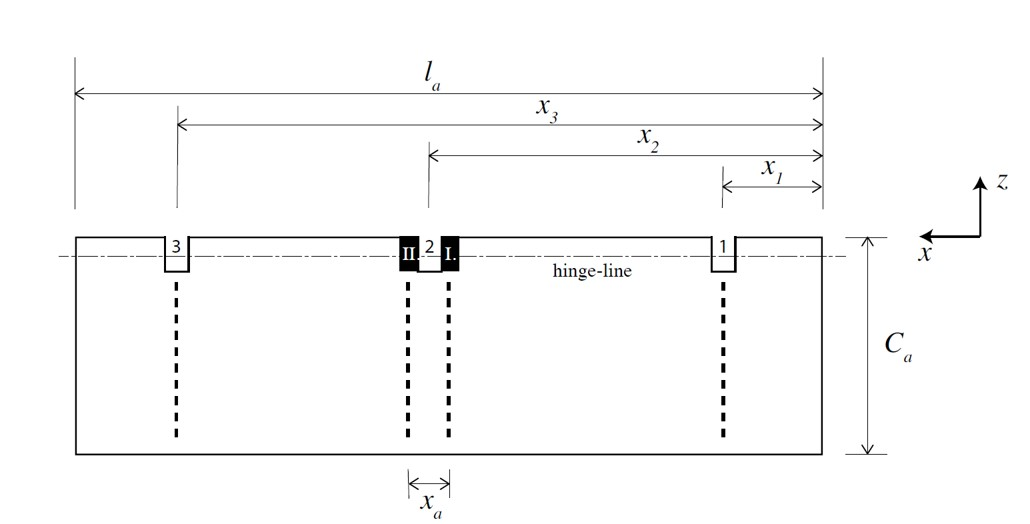
\includegraphics[width=8cm]{Images/Dimension_top_view.jpg}
\caption{Geometry and dimensions: Top view \cite{Assignment_description}.}
\label{fig:Dimensions_top_view}
\end{minipage}
\hspace{0.5cm}
\begin{minipage}[b]{0.45\linewidth}
\centering
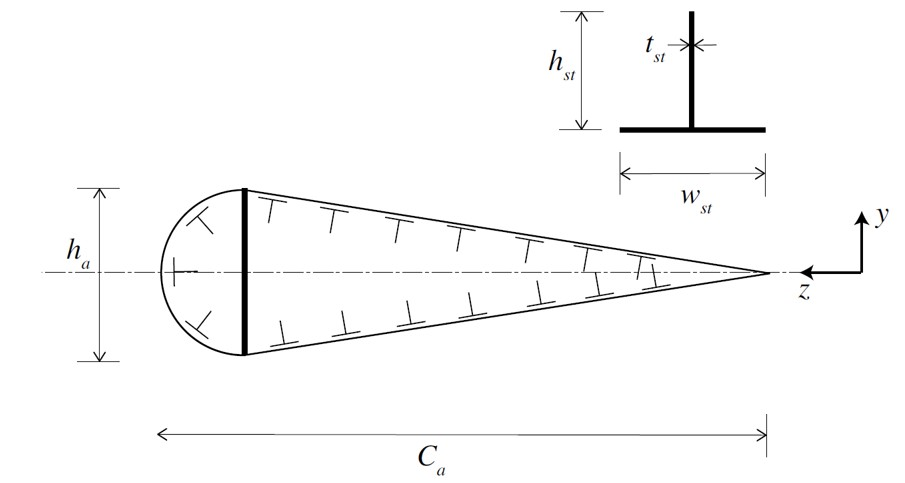
\includegraphics[scale=0.1]{Images/Dimension_side_view.jpg}
\caption{Geometry and dimensions: Side view \cite{Assignment_description}. }
\label{fig:Dimensions_side_view}
\end{minipage}
\begin{minipage}[b]{\linewidth}
\centering
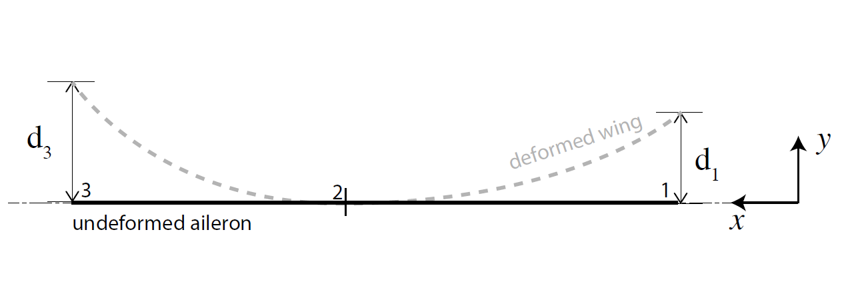
\includegraphics[width=7.5cm]{Images/Dimension_back_view.jpg}
\caption{Geometry of the deformed and undeformed aileron : Back view \cite{Assignment_description}.}
\label{fig:Dimensions_back_view}
\end{minipage}
\end{figure}

\begin{table}[]
\caption{Parameters of aileron of the Fokker 100 \cite{aircraft_data}}
\label{ParametersaileronF100}
\begin{tabular}{|l|l|l|l|}
\hline
\textbf{Property}                                                                       & \textbf{Symbol} & \textbf{Value} & \textbf{Unit} \\ \hline
Chord length aileron                                                           & C\_a   & 0.505 & m    \\ \hline
Span of the aileron                                                            & l\_a   & 1.611 & m    \\ \hline
x-location of hinge 1                                                          & x\_1   & 0.125 & m    \\ \hline
x-location of hinge 2                                                          & x\_2   & 0.498 & m    \\ \hline
x-location of hinge 3                                                          & x\_3   & 1.494 & m    \\ \hline
Distance between actuator 1 and 2                                              & x\_a   & 24.5  & cm   \\ \hline
Aileron height                                                                 & h      & 16.1  & cm   \\ \hline
Skin thickness                                                                 & t\_sk  & 1.1   & mm   \\ \hline
Spar thickness                                                                 & t\_sp  & 2.4   & mm   \\ \hline
Thickness of stiffener                                                         & t\_st  & 1.2   & mm   \\ \hline
Height of stiffener                                                            & h\_st  & 1.3   & cm   \\ \hline
Width of stiffener                                                             & w\_st  & 1.7   & cm   \\ \hline
Number of stiffeners (equally spaced along the periphery of the cross-section) & n\_st  & 11    & -    \\ \hline
Vertical displacement hinge 1                                                  & d\_1   & 0.389 & cm   \\ \hline
Vertical displacement hinge 3                                                  & d\_3   & 1.245 & cm   \\ \hline
Maximum upward deflection                                                      & \theta      & 30    & deg  \\ \hline
Load in actuator 2                                                             & P      & 49.2  & kN   \\ \hline
\end{tabular}
\end{table}






\subsection{Load case and free body diagrams}
The locations of the three hinges and the two actuators can be seen in \figautoref{fig:Dimensions_top_view}.
The aileron is attached to the wing via three hinges, numerically ordered from right to left in \figautoref{fig:Dimensions_top_view}. The second (middle) hinge is fixed in x-,y- and z-direction.
The first (right) and second (left) hinge are fixed only in y-direction.
The actuator that is numbered I in \figautoref{fig:Dimensions_top_view} is fixed.
At each hinge there are three reaction forces in x-,y- and z-direction. \\

\noindent A point load P acts at actuator II in negative y- and z-direction. Its direction is equal to a negative rotation around the x-axis that is equal to the maximum upward deflection angle. 
A distributed load q is present due to aerodynamic forces. Its direction is in negative y-direction, perpendicular to the symmetry plane of the aileron (x-,z-plane). The magnitude of the distributed load varies over the aileron surface in both x- and z-direction. 

\noindent These loads acting on the aileron in the relevant loading case can now be visualised. This is done in the free body diagrams for the top view, side view and back view. These can be seen in \figautoref{fig:FBD_top_view}, \figautoref{fig:FBD_side_view} and \figautoref{fig:FBD_back_view}.
\par
\begin{figure}[H]
\begin{minipage}[b]{0.45\linewidth}
\centering
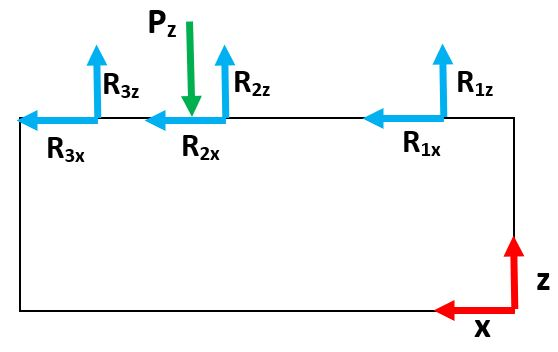
\includegraphics[width=6cm]{Images/New_FBD_top.JPG}
\caption{Free body diagram: Top view}
\label{fig:FBD_top_view}
\end{minipage}
\hspace{0.5cm}
\begin{minipage}[b]{0.45\linewidth}
\centering
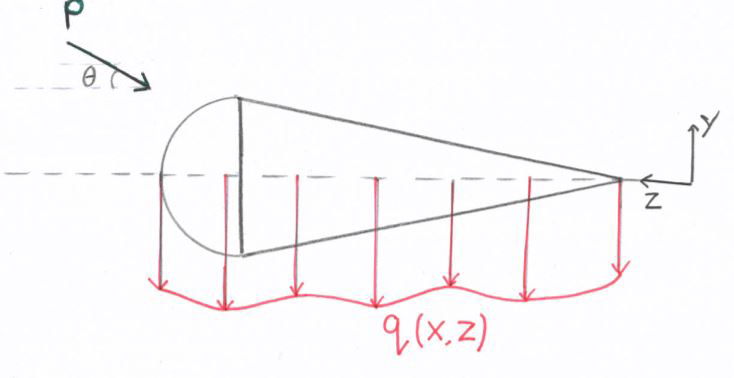
\includegraphics[width=0.95\textwidth]{Images/FBD_side_view.jpg}
\caption{Free body diagram: Side view}
\label{fig:FBD_side_view}
\end{minipage}
\begin{minipage}[b]{\linewidth}
\centering
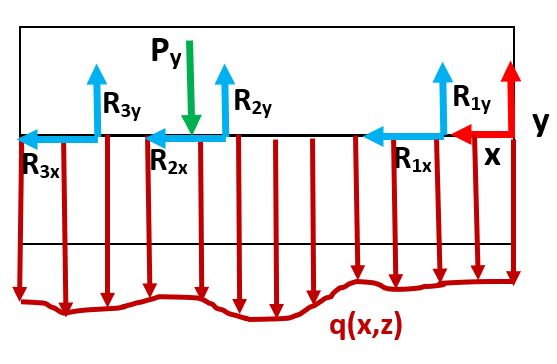
\includegraphics[width=5cm]{Images/New_FBD_back_view.JPG}
\caption{Free body diagram: Back view}
\label{fig:FBD_back_view}
\end{minipage}
\end{figure}
